\section{Linear Relations}

\begin{outline}

\0
\subsection{Algebra reiterated}
	\1 Definitions
		\2 \textbf{Term:} A term is either a single number or a variable, or numbers and variables multiplied together. 
			\3 Examples: $2x$, $4x^7 y$, $\frac{4b}{7}$
		\2 \textbf{Coefficient:} A coefficient is a number used to multiply a variable.
			\3 Examples: $8$ is the coefficient of $x^3$ in $x^3 - 8$
		\2 \textbf{Pronumeral:} A pronumeral is a letter that is used to represent a number which is unknown.
			\3 Examples: $x$, $y$, $z$
		\2 \textbf{Expression:} An expression is a group of terms.
			\3 Examples: $4y$, $7x^2 + 3xy^2$, $\frac{x^2+9}{42}$
		\2 \textbf{Equation:} An equation says that two things are equal. It will always have an equals sign ``$=$'' somewhere, to indicate that the two sides are equal.
			\3 Examples: $9x = 34$, $x = 0$, $\frac{4}{x}=32$, $4^x=16$
	\1 Algebraic techniques
		\2 \textbf{Like terms}
			\3 Like terms are terms that have the same pronumeral, which represents the same number. Using addition and subtraction, like terms can be collected into a single term.
				\[5x-3x+x => 3x\]
		\2 \textbf{Distributive law}
			\3 The distributive law is used to expand brackets.
				\[a(b+c) => ab+ac\]
				\[a(b-c) => ab - ac\]
		\2 \textbf{Factorisation}
			\3 Many expressions can be factorised by taking out the highest common factor.
				\[4x-16 = 4(x-4)\]
				\[2x^2 + 4x^3 = 2x^2(2x+ 1)\]
	\1 General properties
		\2 \textbf{Associative:}
			\[a \times (b \times c) = (a \times b) \times c\]
			\[a + (b + c) = (a + b) + c\]
		\2 \textbf{Commutative:}
			\[ab = ba\]
			\[a + b = b + a\]
			\[\frac{a}{b}\ne\frac{b}{a}\]
			\[a - b \ne b - a\]
		\2 \textbf{Identity:}
			\[a \times 1 = a\]
			\[a + 0 = a\]
		\2 \textbf{Inverse:}
			\[a \times \frac{1}{a} = 1\]
			\[a + (-a) = 0\]

\0
\subsection{Algebraic fractions}
	\1 Simplifying algebraic fractions
		\2 The easiest ways to simplify algebraic fractions are by factorising expressions where possible and cancelling any common factors. Once this is complete, it becomes much easier to complete any necessary calculations, such as adding, subtracting, multiplying, or dividing.
			\3 Examples
				\[\frac{6x^3 y}{2xy} = \frac{\cancelto{3}{6} \times \cancelto{x^2}{x^3} \times \cancelto{1}{y}}{\cancelto{1}{2}\times \cancelto{1}{x} \times \cancelto{1}{y}} = 3x^2\]
				\[\frac{5-25x}{5} = \frac{5(1-5x)}{5} = \frac{\cancelto{1}{5}(1-5x)}{\cancelto{1}{3}} = 1-5x\]
	\1 Adding and subtracting algebraic fractions
		\2 Adding and subtracting algebraic fractions is as simple as expressing the fractions in terms of their lowest common denominator, and then combining the numerator. After combining the numerator, it is necessary to check if the equation can be simplified, and simplify the equation to its simplest form if possible.
			\3 Examples
				\[\frac{4}{5}+\frac{10}{4} = \frac{16}{20}+\frac{50}{20} = \frac{66}{20} = \frac{33}{10}\]
	\1 Multiplying algebraic fractions
		\2 When multiplying algebraic fractions, first look for any factors that can be cancelled, and factorise any expressions fit for factorisation. Then, multiply the numerators together and the denominators together.
			\3 Examples
				\[\frac{6}{x}\times\frac{6+x}{12} = \frac{\cancelto{1}{6}}{x}\times\frac{6+x}{\cancelto{2}{12}} = \frac{6+x}{2x}\]
	\1 Dividing algebraic fractions
		\2 The division of algebraic fractions is very simple. Flipping one of the two fractions will change the calculation from division to multiplication.
			\3 Method
				\[\frac{a}{b}\div\frac{c}{d} = \frac{a}{b}\times\frac{d}{c}\]
	\1 Adding and subtracting complex algebraic fractions
		\2 Adding and subtracting complex algebraic fractions involves inspecting the problem to see if there are any factors, possible factorisations, or simplifications. Often the first step will be to find the lowest common multiple or denominator.
			\3 Examples
				\[\frac{3}{x-6}-\frac{2}{x-2} = \frac{3(x+2)}{(x-6)(x+2)}-\frac{2(x-6)}{(x-6)(x+2)}\]
				\[= \frac{3(x+2)-2(x-6)}{(x-6)(x+2)}\]
				\[= \frac{3x+6-2x+12}{(x-6)(x+2)}\]
				\[= \frac{x+18}{(x-6)(x+2)}\]

\0
\subsection{Solving linear equations}
	\1 Solving linear equations
		\2 A linear equation is a statement that contains an equals sign and includes a variable raised to the power of 1. Ther must be no other powers. The useful steps in solving linear equations are using linear operations (backtracking), collecting like terms, expanding brackets, and multiplying by the lowest common denominator. Checking the solution is also simple using substitution. One can replace the $x$ in the equation with the solution one finds, and evaluate the expression to check the accuracy of the answer.
			\3 Examples
				\[4x+5=17\]
				\[4x = 12\]
				\[x = 3\]
				\[\text{Check: } 4\times 3 + 5 = 17\]
	\1 Solving linear equations involving algebraic fractions
		\2 Essential to solving equations involving algebraic fractions is realising that fractions are just divisions. That way, equations can be evaluated in the same way as any other linear equation.
			\3 Examples
				\[\frac{4x-2}{3}=\frac{3x-1}{2}\]
				\[\frac{\cancelto{2}{6}(4x-2)}{\cancelto{1}{3}} = \frac{\cancelto{3}{6}(3x-1)}{\cancelto{1}{2}}\]
				\[2(4x-2)=3(3x-1)\]
				\[8x-4=9x-3\]
				\[-4=x-3\]
				\[-1=x\]
				\[\therefore x = -1\]
				\[\frac{4\times(-1)-2}{3}=\frac{3\times(-1)-1}{2}\]

\0				
\subsection{Inequalities}
	\1 Inequality signs
		\2 $x > a$ means $x$ is greater than $a$.
\begin{center}
\begin{tikzpicture}[scale=3]
\draw[black, arrows={-Triangle[angle=90:4pt,black,fill=black]}]  (0,0) -- (-1,0);
\draw[black, arrows={-Triangle[angle=90:4pt,black,fill=black]}]  (0,0) -- (1,0) node[anchor=west]{$x$};
\draw[black, arrows={-Triangle[angle=90:4pt,black,fill=black]}]  (0,0.1) -- (0.8,0.1);
\draw (0,0) -- (0,-0.05) node[anchor=north]{$a$};
\filldraw[fill=white, draw=black] (0,0.1) circle (0.03);
\end{tikzpicture}
\end{center}
		\2 $x \geq a$ means $x$ is greater than or equal to $a$.
\begin{center}
\begin{tikzpicture}[scale=3]
\draw[black, arrows={-Triangle[angle=90:4pt,black,fill=black]}]  (0,0) -- (-1,0);
\draw[black, arrows={-Triangle[angle=90:4pt,black,fill=black]}]  (0,0) -- (1,0) node[anchor=west]{$x$};
\draw[black, arrows={-Triangle[angle=90:4pt,black,fill=black]}]  (0,0.1) -- (0.8,0.1);
\draw (0,0) -- (0,-0.05) node[anchor=north]{$a$};
\filldraw[fill=black, draw=black] (0,0.1) circle (0.03);
\end{tikzpicture}
\end{center}
		\2 $x < a$ means $x$ is less than $a$.
\begin{center}
\begin{tikzpicture}[scale=3]
\draw[black, arrows={-Triangle[angle=90:4pt,black,fill=black]}]  (0,0) -- (-1,0);
\draw[black, arrows={-Triangle[angle=90:4pt,black,fill=black]}]  (0,0) -- (1,0) node[anchor=west]{$x$};
\draw[black, arrows={-Triangle[angle=90:4pt,black,fill=black]}]  (0,0.1) -- (-0.8,0.1);
\draw (0,0) -- (0,-0.05) node[anchor=north]{$a$};
\filldraw[fill=white, draw=black] (0,0.1) circle (0.03);
\end{tikzpicture}
\end{center}
		\2 $x \leq a$ means $x$ is less than or equal to $a$.
\begin{center}
\begin{tikzpicture}[scale=3]
\draw[black, arrows={-Triangle[angle=90:4pt,black,fill=black]}]  (0,0) -- (-1,0);
\draw[black, arrows={-Triangle[angle=90:4pt,black,fill=black]}]  (0,0) -- (1,0) node[anchor=west]{$x$};
\draw[black, arrows={-Triangle[angle=90:4pt,black,fill=black]}]  (0,0.1) -- (-0.8,0.1);
\draw (0,0) -- (0,-0.05) node[anchor=north]{$a$};
\filldraw[fill=black, draw=black] (0,0.1) circle (0.03);
\end{tikzpicture}
\end{center}
		\2 $a < x \leq b$ could be illustrated as shown.
\begin{center}
\begin{tikzpicture}[scale=3]
\draw[black, arrows={-Triangle[angle=90:4pt,black,fill=black]}]  (0,0) -- (-1,0);
\draw[black, arrows={-Triangle[angle=90:4pt,black,fill=black]}]  (0,0) -- (1,0) node[anchor=west]{$x$};
\draw (0.8,0.1) -- (-0.8,0.1);
\draw (-0.8,0) -- (-0.8,-0.05) node[anchor=north]{$a$};
\draw (0.8,0) -- (0.8,-0.05) node[anchor=north]{$b$};
\filldraw[fill=white, draw=black] (-0.8,0.1) circle (0.03);
\filldraw[fill=black, draw=black] (0.8,0.1) circle (0.03);
\end{tikzpicture}
\end{center}
	\1 Rules for solving inequalities
		\2 With inequalities, they follow similar rules to solving linear equations, except for two important rules. When multiplying or dividing by a negative number one must reverse the inequality sign. If the sides are switched, one must also reverse the inequality sign.
	\1 Solving inequalities
		\2 When solving inequalities, unless multiplying or dividing by a negative or switching the sides, one must treat the inequality sign as if it is an equals sign. This means that when an operation is completed on one side, the same operation must be completed on the other side.
			\3 Examples
				\[\text{Example One: }3x + 4 > 13\]
				\[3x > 9\]
				\[\therefore x > 3\]
				
				\[\text{Example Two: }4-\frac{x}{3}\leq 6\]
				\[-\frac{x}{3}\leq 2\]
				\[\therefore x \geq -6\]

\0
\subsection{Graphing straight lines}
	\1 Definitions
		\2 The gradient, $m$, is a number that describes the slope of a line. A zero gradient is horizontal, an infinite gradient is vertical. A positive gradient goes upwards from $x$ negative to $x$ positive, while a negative gradient goes downwards from $x$ negative to $x$ positive.
			\[gradient = m = \frac{rise}{run}\]
		\2 The intercepts are the points where the line crosses the $x$-axis and the $y$-axis.
			\3 The $y$-intercept is where $x$ = 0.
			\3 The $x$-intercept is where $y$ = 0.
	\1 Special lines
		\2 Special lines include those with only one axis intercept, and those with their two axis intercepts both at the origin.
			\3 horizontal lines $y = c$ where c is the $y$-intercept
			\3 vertical lines $x = k$ where k is the $x$-intercept
			\3 lines passing through the origin $y = mx$
	\1 Common forms of straight line (linear) equations
		\2 The gradient-intercept form of a straight line is $y = mx + c$ where $m$ is the gradient and $c$ is the $y$-coordinate of the $y$-intercept.
		\2 In two dimensions, straight line graphs can be represented with linear equations. The common forms of linear equations are $y = mx+c$ and $ax+by=d$ where $a, b, c, d$ and $m$ are constants. From linear equations graphs can be drawn.
			\3 Examples
			\3 Shown is $y = -2$, $x = -2$, and $y = \frac{1}{2}x$
\begin{center}
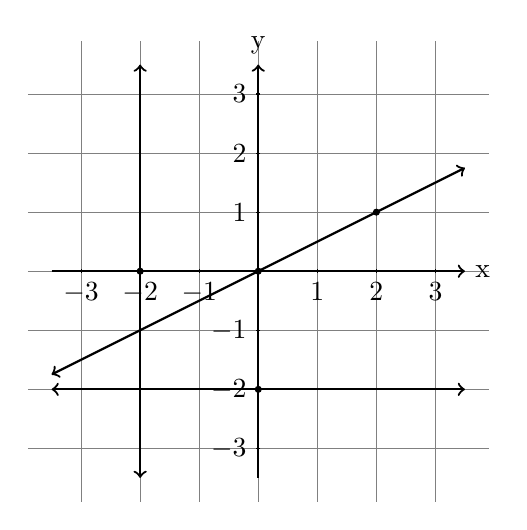
\begin{tikzpicture}[scale=0.75]
\draw[step=1cm,gray,very thin] (-3.9,-3.9) grid (3.9,3.9);
\foreach \x in {-3,-2,-1,1,2,3}
	\draw (\x cm,1pt) -- (\x cm,-1pt) node[anchor=north] {$\x$};
\foreach \y in {-3,-2,-1,1,2,3}
	\draw (1pt,\y cm) -- (-1pt,\y cm) node[anchor=east] {$\y$};
\draw[thick,->] (-3.5,0) -- (3.5,0) node[anchor=west] {x};
\draw[thick,->] (0,-3.5) -- (0,3.5) node[anchor=south] {y};
\draw[thick,<->] (-2,-3.5) -- (-2,3.5);
\draw[thick,<->] (-3.5,-2) -- (3.5,-2);
\draw[thick,<->] (-3.5,-1.75) -- (3.5,1.75);
\filldraw[fill=black, draw=black] (-2,0) circle (0.05);
\filldraw[fill=black, draw=black] (0,-2) circle (0.05);
\filldraw[fill=black, draw=black] (2,1) circle (0.05);
\filldraw[fill=black, draw=black] (0,0) circle (0.05);
\end{tikzpicture}
\end{center}
	\1 Deciding if a point is on a line
		\2 In the form $y = mx + c$, one must substitute the $x$ and $y$ coordinates of the point into the equation. If the equation is equal, the point must be on the line.
			\3 Examples -- Using the point $(-2, 7)$
				\[\text{Example One: }y = -3x + 1\]
				\[7 = -3(-2) + 1\]
				\[7 = 7\]
				\[\therefore (-2,7) \text{ is on the line.}\]
				
				\[\text{Example Two: }2x+2y=1\]
				\[2(-2) + 2(7) = 1\]
				\[-4 + 14 = 1\]
				\[10 \ne 1\]
				\[\therefore (-2, 7) \text{ is not on the line.}\]
	\1 Finding $x$- and $y$-intercepts from linear equations
		\2 To find the $x$-intercept, one needs to substitute $y$ with $0$, as the $x$-intercept is at $y=0$. Once $0$ is substituted in, solving the equation will find the $x$-intercept. To find the $y$-intercept, the reverse is necessary. One must substitute $x$ with $0$, as the $y$-intercept is at $x=0$. Once one has substituted $0$ in, solving the equation will yield the $y$-intercept.
			\3 Examples
				\[\text{Example One: }y = 2x - 8\]
				\[y\text{-intercept } (x=0):\]
				\[y = 2(0) - 8\]
				\[y = -8\]
				\[\text{The }y\text{-intercept is }{-8}\]
				\[x\text{-intercept } (y=0):\]
				\[0 = 2x - 8\]
				\[8 = 2x\]
				\[x = 4\]
				\[\text{The }x\text{-intercept is }4\]
				
				\[\text{Example Two: }-3x - 2y = 6\]
				\[y\text{-intercept }(x=0):\]
				\[-3(0) - 2y = 6\]
				\[-2y = 6\]
				\[y = -3\]
				\[\text{The }y\text{-intercept is }{-3}\]
				\[x\text{-intercept } (y=0):\]
				\[-3x - 2(0) = 6\]
				\[-3x = 6\]
				\[x = -2\]
				\[\text{The }x\text{-intercept is }{-2}\]

\0
\subsection{Finding a rule for a linear graph}
	\1 Finding the gradient of a line
		\2 To determine the gradient of a line, one must have the coordinates of two points. Preferably one of the points is the $y$-intercept, but this is only necessary if one wants to find the rule and not just the gradient. The rule to find the gradient is the difference between two $y$-coordinates ``$y_2$'' and ``$y_1$'', divided by the difference between two $x$-coordinates ``$x_2$'' and ``$x_1$''.
			\3 Equation
				\[m = \frac{y_2 - y_1}{x_2 - x_1}\]
				\[\text{where }(x_1, y_1)\text{ and }(x_2, y_2)\text{ are points on the line}\]
				
	\1 Finding the equation of a line given the $y$-intercept and a point.
		\2 Using the $y$-intercept and a point, one can find the equation of a line. Using the $m = \frac{y_2 - y_1}{x_2 - x_1}$ equation where $(x_1, y_1)$ is the $x$-intercept, one can easily substitute $x_1$ as $c$ in the equation $y = mx + c$. With $m$ and $c$ constructed, one is able to construct a full equation.
			\3 Equation
				\[y = \left(\frac{y_2 - y_1}{x_2 - x_1}\right)x + (y_1)\]
 
\0
\subsection{Length and midpoint of a line segment}
	\1 Length of a line segment
		\2 The length of a line segment is found using a variant of the Pythagoras' theorem. It involves finding the difference between $y_2$ and $y_1$, and $x_2$ and $x_1$, squaring them individually, adding them together, and then performing a square root on the sum.
			\3 Equation
				\[d = \sqrt{(x_2 - x_1)^2 + (y_2 - y_1)^2}\]
				
	\1 Midpoint of a line segment
		\2 The midpoint of a line segment, known as $M$, is the point exactly halfway in between two points $(x_1, y_1)$ and $(x_2, y_2)$.
			\3 Equation
				\[M = \left(\frac{x_1 + x_2}{2}, \frac{y_1 + y_2}{2}\right)\]

\0
\subsection{Perpendicular and parallel lines}
	\1 Parallel Postulate
		\2 ``It is true that if a straight line falling on two straight lines makes the interior angles on the same side less than two right angles, the two straight lines, if produced indefinitely, intersect on that side on which are the angles less than the two right angles.'' --Euclid of Alexandria
	\1 Explanation
		\2 If a straight line is placed in a perpendicular position across two lines, and the cointerior angles do not sum to 180\degree, the two lines are not parallel.
	\1 How to determine parallel and perpendicular lines
		\2 Two parallel lines have the same gradient. Two perpendicular lines with gradients $m_1$ and $m_2$ will adhere to the following rules (it is not necessary to test both):
			\[m_1 \times m_2 = -1\]
			\[m_2 = -\frac{1}{m_1}\]

\0
\subsection{Simultaneous equations - substitution}
	\1 What are simultaneous equations
		\2 Simultaneous equations are a set of equations, where the goal is generally to find the point where the graphs of the two equations meet. The two equations must be non-parallel, as there is no point of intersection in a set of parallel equations.
	\1 Substitution
		\2 Solving a simultaneous equation can be done in two ways. Using the substitution method is usually due to at least one of the equations having one variable as the subject. The substitution method involves substituting one equation into the other, followed by solving the equation to yield the other variable. That variable can be substituted back into the equation, to solve the first variable.
			\3 Examples
%WATCH THE FORMATTING HERE - SPACES ARE KINDA SCREWY
				\[(1)\ \ \ \ \ \ \ \ y = 3x + 2\]
				\[(2)\ \ \ \ \ \ \ \ y = 7x - 8\]
				\[\text{Substitute equation (2) into equation (1)}\]
				\[7x - 8 = -3x + 2\]
				\[10x = 10\]
				\[x = 1\]
				\[\text{Substitute $x = 1$ into equation (1)}\]
				\[y = -3(1) + 2\]
				\[y = -1\]
				\[\text{Solution is }(1, -1)\]
				
\0
\subsection{Simultaneous equations - elimination}
	\1 What are simultaneous equations
		\2 Simultaneous equations are a set of equations, where the goal is generally to find the point where the graphs of the two equations meet. The two equations must be non-parallel, as there is no point of intersection in a set of parallel equations.
	\1 Elimination
		\2 The method of elimination as a way of solving simultaneous equations is often used when both equations are in the form of $ax + by = d$. The elimination method involves adding or subtracting two equations to eliminate one of the two variables in the result. If there are no ways to eliminate them, often multiplying one can help in eliminating the variable in question.
			\3 Examples
%WATCH THE FORMATTING HERE - SPACES ARE KINDA SCREWY
				\[(1)\ \ \ \ \ \ \ \ y - 3x = 1\ \ \ \]
				\[(2)\ \ \ \ \ \ \ \ 2y - 5x = 13\]
				\[(1)\times2 => (3)\ \ \ \ \ \ \ \ 2y - 6x = 2\ \ \ \ \ \ \ \ \ \ \ \ \ \ \ \ \ \]
				\[(2)-(3)\ \ \ \ \ \ \ \ 11x = 11\ \ \ \ \ \ \ \ \ \ \ \ \]
				\[\ \ \ x = 1\]
				\[\ \ \ \ \ \ \ \ \ \ \ \ \text{Substitute $x = 1$ into equation (1)}\]
				\[\ \ \ \ \ \ \ \ \ \ \ \ \ y - 3(1) = 1\]
				\[\ \therefore y = 4\]
				\[\text{Solution is }(1,4)\ \ \ \ \ \ \ \ \ \ \ \]
				
\0
\subsection{Further applications of simultaneous equations}
	\1 Setting up and solving simultaneous equations
		\2 Setting up a simultaneous equation is the process of finding two solvable equations from text. One must define a variable for each unknown, write down two equations from the information given, solve the equations simultaneously to find the solution, and interpret the solution and answer the question in words.
			\3 Example
%WATCH THE FORMATTING HERE - SPACES ARE KINDA SCREWY

				The sum of the ages of two children is 17 and the difference in their ages is 5. If Kara is the older sister of Ben, determine their ages.
				
				\[\text{Let $k$ be Kara's age and $b$ be Ben's age}\]
				\[(1)\ \ \ \ \ \ \ \ k + b = 17\]
				\[(2)\ \ \ \ \ \ \ \ k - b = 5\ \]
				\[\ \ (1)+(2)\ \ \ \ \ \ \ \ 2k = 22\ \ \ \ \ \ \ \ \ \ \ \ \]
				\[\ \ \ \ \ \therefore k = 11\]
				\[\text{Substitute } k = 11 \text{ into equation } (1)\]
				\[\ \ \ \ \ \ \ \ \ \ \ \ \ \ 11 + b = 17\]
				\[\ \ \ \ \therefore b = 5\]
	\1 Solving further applications with two variables
		\2 To solve further applications with two variables, the elimination method of solving simultaneous equations is ideal to use.
			\3 Example
%WATCH THE FORMATTING HERE - SPACES ARE KINDA SCREWY

				John buys 3 daffodils and 5 petunias from the nursery and pays \$25. Julia buys 4 daffodils and 3 petunias for \$26. Determine the cost of each type of flower.
				
				\[\text{Let \$$d$ be the cost of a daffodil and \$$p$ be the cost of a petunia}\]
				\[\]
				\[(1)\ \ \ \ \ \ \ \ 3d + 5p = 25\ \]
				\[(2)\ \ \ \ \ \ \ \ 4d + 3p = 26\ \]
				\[(1)\times4 => (3)\ \ \ \ \ \ \ \ 12d + 20p = 100\ \ \ \ \ \ \ \ \ \ \ \ \]
				\[(2)\times3 => (4)\ \ \ \ \ \ \ \ 12d + 9p = 78\ \ \ \ \ \ \ \ \ \ \ \ \ \ \ \]
				\[(3) - 4 =>\ \ \ \ \ \ \ \ 11p = 22\ \ \ \ \ \ \ \ \ \ \ \ \ \ \ \ \ \]
				\[\therefore p = 2\]

\0
\subsection{Half planes}
	\1 Linear equalities
		\2 A linear inequality with one variable can be solved using the same method as solving an inequality.
		\2 The solution to a linear inequality with two variables is illustrated using a half plane.
		\2 If the equation is of the form $ax + by = d$, it is usually simpler to test a point to see which side of the line is included in the region.
		\2 If $y$ is the subject of the inequality follow these simple rules:
			\3 $y \geq mx + c$
				\4 Draw a solid line (as it is included in the region) and shade above.
			\3 $y > mx + c$
				\4 Draw a broken line (as it is included in the region) and shade above.
			\3 $y \leq mx + c$
				\4 Draw a solid line (as it is included in the region) and shade below.
			\3 $y < mx + c$
				\4 Draw a broken line (as it is included in the region) and shade below.
		\2 Examples
\begin{center}
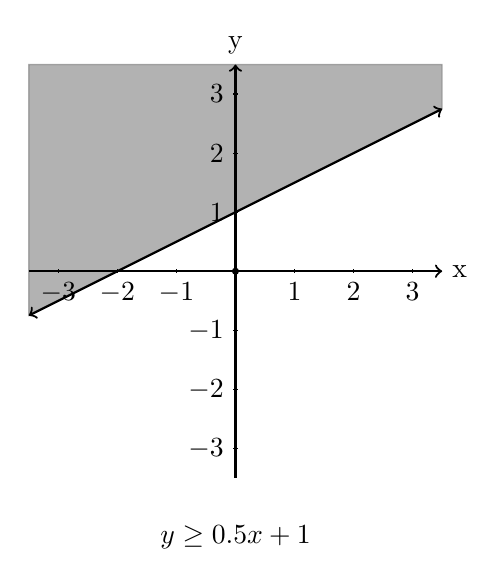
\begin{tikzpicture}[scale=0.75]
\filldraw[fill=black, opacity=0.3] (-3.5,-0.75) -- (3.5,2.75) -- (3.5,3.5) -- (-3.5,3.5) -- cycle;
\foreach \x in {-3,-2,-1,1,2,3}
	\draw (\x cm,1pt) -- (\x cm,-1pt) node[anchor=north] {$\x$};
\foreach \y in {-3,-2,-1,1,2,3}
	\draw (1pt,\y cm) -- (-1pt,\y cm) node[anchor=east] {$\y$};
\draw[thick,->] (-3.5,0) -- (3.5,0) node[anchor=west] {x};
\draw[thick,->] (0,-3.5) -- (0,3.5) node[anchor=south] {y};
\draw[thick,<->] (-3.5,-0.75) -- (3.5,2.75);
\filldraw[fill=black, draw=black] (0,0) circle (0.05);
\node at (0, -4.5){$y \geq 0.5x + 1$};
\end{tikzpicture}
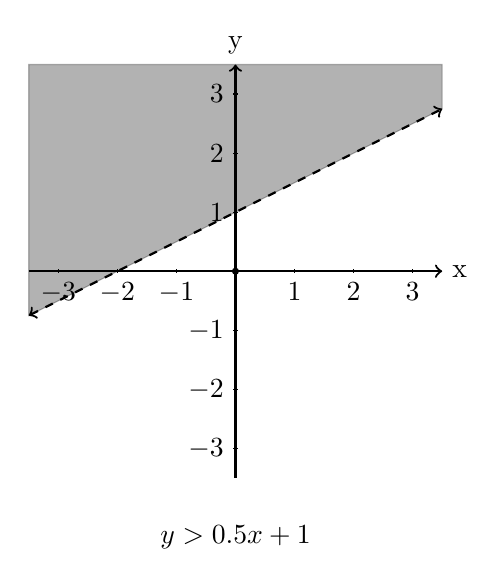
\begin{tikzpicture}[scale=0.75]
\filldraw[fill=black, opacity=0.3] (-3.5,-0.75) -- (3.5,2.75) -- (3.5,3.5) -- (-3.5,3.5) -- cycle;
\foreach \x in {-3,-2,-1,1,2,3}
	\draw (\x cm,1pt) -- (\x cm,-1pt) node[anchor=north] {$\x$};
\foreach \y in {-3,-2,-1,1,2,3}
	\draw (1pt,\y cm) -- (-1pt,\y cm) node[anchor=east] {$\y$};
\draw[thick,->] (-3.5,0) -- (3.5,0) node[anchor=west] {x};
\draw[thick,->] (0,-3.5) -- (0,3.5) node[anchor=south] {y};
\draw[thick,<->, dashed] (-3.5,-0.75) -- (3.5,2.75);
\filldraw[fill=black, draw=black] (0,0) circle (0.05);
\node at (0, -4.5){$y > 0.5x + 1$};
\end{tikzpicture}
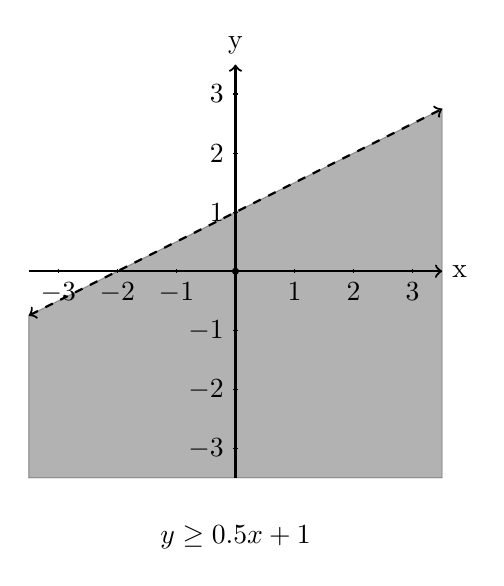
\begin{tikzpicture}[scale=0.75]
\filldraw[fill=black, opacity=0.3] (-3.5,-0.75) -- (3.5,2.75) -- (3.5,-3.5) -- (-3.5,-3.5) -- cycle;
\foreach \x in {-3,-2,-1,1,2,3}
	\draw (\x cm,1pt) -- (\x cm,-1pt) node[anchor=north] {$\x$};
\foreach \y in {-3,-2,-1,1,2,3}
	\draw (1pt,\y cm) -- (-1pt,\y cm) node[anchor=east] {$\y$};
\draw[thick,->] (-3.5,0) -- (3.5,0) node[anchor=west] {x};
\draw[thick,->] (0,-3.5) -- (0,3.5) node[anchor=south] {y};
\draw[thick,<->, dashed] (-3.5,-0.75) -- (3.5,2.75);
\filldraw[fill=black, draw=black] (0,0) circle (0.05);
\node at (0, -4.5){$y \geq 0.5x + 1$};
\end{tikzpicture}
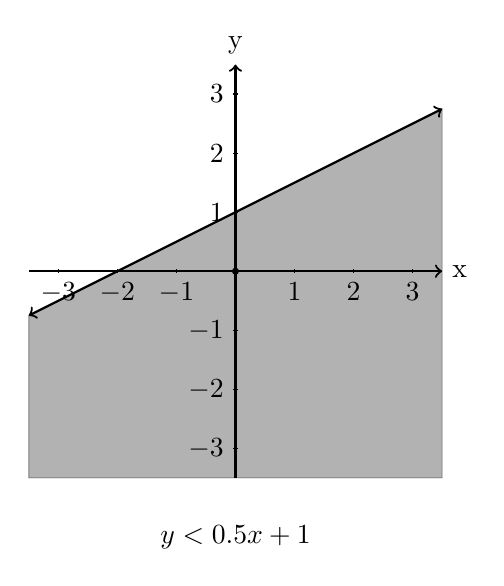
\begin{tikzpicture}[scale=0.75]
\filldraw[fill=black, opacity=0.3] (-3.5,-0.75) -- (3.5,2.75) -- (3.5,-3.5) -- (-3.5,-3.5) -- cycle;
\foreach \x in {-3,-2,-1,1,2,3}
	\draw (\x cm,1pt) -- (\x cm,-1pt) node[anchor=north] {$\x$};
\foreach \y in {-3,-2,-1,1,2,3}
	\draw (1pt,\y cm) -- (-1pt,\y cm) node[anchor=east] {$\y$};
\draw[thick,->] (-3.5,0) -- (3.5,0) node[anchor=west] {x};
\draw[thick,->] (0,-3.5) -- (0,3.5) node[anchor=south] {y};
\draw[thick,<->] (-3.5,-0.75) -- (3.5,2.75);
\filldraw[fill=black, draw=black] (0,0) circle (0.05);
\node at (0, -4.5){$y < 0.5x + 1$};
\end{tikzpicture}
\end{center}

	\1 Sketching half planes
		\2 To sketch a half plane, one must find the $x$- and $y$- intercepts, and mark them on a graph. From there, one is able to draw the complete line of the graph. If the $x$- and $y$- intercepts are both at zero, one must substitute in a value other than 0 into the $x$ or $y$ co-efficient, and calculate the equation. The result, combined with the 
	\1 Finding the intersecting region

\end{outline}
